\section{Bridge}

O padrão Bridge permite variar as abstrações e as 
implementações de uma solução de forma independente, 
definindo uma interface que serve como ponte entre ambas. 
As operações da implementação são delegadas para essa 
nova interface, permitindo que as abstrações sejam 
implementadas sem precisar conhecer o tipo de 
implementação que está sendo utilizado. A estrutura do 
padrão pode ser vista na figura \ref{bridge_struct}.\cite{gamma:1995}

\begin{figure}[htb]
	\caption{\label{bridge_struct}Estrutura do Bridge}
	\begin{center}
	    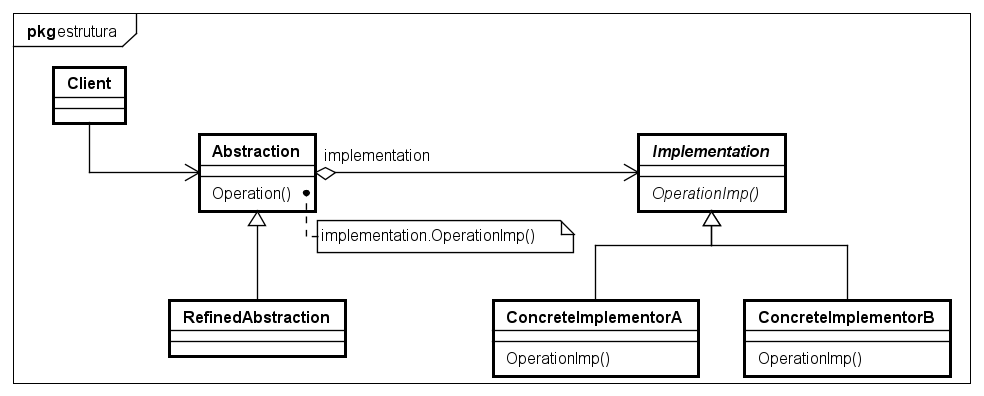
\includegraphics[scale=0.5]{5_padroes-contexto-funcional/5.2_estruturais/5.2.2_bridge/bridge_estrutura.png}
	\end{center}
\end{figure}

\subsection*{Exemplo Orientado a Objetos}

Como exemplo, pode ser considerada a implementação de 
uma janela em um \textit{toolkit} para construir interfaces 
de usuários que permite o uso de implementações diferentes 
de janela: PM e XWindow. Além disso, é preciso definir tipos 
diferentes de janela, como janelas para ícones e janelas 
transitórias. Para que não seja necessário implementar 
uma versão diferente de janela de ícone e transitória 
para cada implementação diferente de janela, o padrão 
Bridge pode ser usado para separar a implementação 
da abstração em duas hierarquias diferentes. O diagrama 
de classes da figura \ref{bridge_exemplo} e o código 
\ref{oobridge} demonstram o uso do padrão para esse 
exemplo.

\begin{figure}[htb]
	\caption{\label{bridge_exemplo}Exemplo de Bridge}
	\begin{center}
	    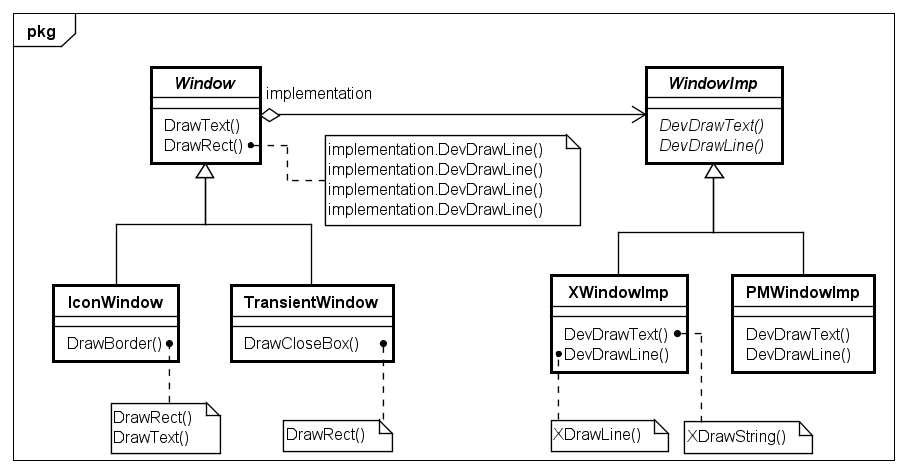
\includegraphics[scale=0.5]{5_padroes-contexto-funcional/5.2_estruturais/5.2.2_bridge/bridge_exemplo.png}
	\end{center}
\end{figure}

\begin{lstlisting}[caption={Bridge Orientado a Objetos},label=oobridge]

abstract class Window(imp : WindowImp) {
  def DrawText() : Unit = {
    imp.DevDrawText()
  }

  def DrawRect() : Unit = {
    imp.DevDrawLine()
    imp.DevDrawLine()
    imp.DevDrawLine()
    imp.DevDrawLine()
  }
}

class IconWindow(imp : WindowImp) extends Window(imp) {
  def DrawBorder() : Unit = {
    DrawRect()
    DrawText()
  }
}

class TransientWindow(imp : WindowImp) extends Window(imp){
  def DrawCloseBox() : Unit = {
    DrawRect()
  }
}

trait WindowImp {
  def DevDrawText()
  def DevDrawLine()
}

class XWindowImp extends WindowImp {
  def DevDrawText() : Unit = {
    //Desenha texto para janela X
  }
  def DevDrawLine() : Unit = {
    //Desenha linha para janela X
  }
}

class PMWindowImp extends WindowImp {
  def DevDrawLine(): Unit = {
    //Desenha linha para janela PM
  }
  def DevDrawText(): Unit = {
    //Desenha texo para janela PM
  }
}

\end{lstlisting}


\subsection*{Contexto Funcional}

Funções de alta ordem também podem ser utilizadas 
para separar as abstrações das implementações. 
No código \ref{fpbridgeabs}, são definidas nas 
linhas 2 e 10, respectivamente, as 
duas funções equivalentes aos métodos das 
classes IconWindow e TransientWindow do exemplo 
orientado a objetos. Ao invés de reutilizar 
funções de uma superclasse, as funções 
DrawText e DrawRect são recebidas por parâmetro.

\begin{lstlisting}[caption={Abstrações no Bridge Funcional},label=fpbridgeabs]
    
def DrawIconBorder(text : String,
                   height : Int, width : Int,
                   DrawText : String => Unit,
                   DrawRect : (Int, Int) => Unit) : Unit = {
  DrawText(text)
  DrawRect(height, width)
}

def DrawTransientCloseBox(height : Int, width : Int,
                          DrawRect : (Int, Int) => Unit) : Unit = {
  DrawRect(height, width)
}
    
\end{lstlisting}

No código \ref{fpbridgeimp}, são definidas as 
funções referentes às implementações diferentes 
de Window. Essas são as funções que podem ser 
passadas como parâmetro para as funções vistas 
no código \ref{fpbridgeabs}. Dessa forma, as 
abstrações de Window tornam-se independentes 
da forma como ela é implementada, resolvendo 
o problema encontrado pelo padrão.

\begin{lstlisting}[caption={Implementações no Bridge Funcional},label=fpbridgeimp]
    
def XDrawLine(size : Int) : Unit = {
  // Desenha linha
}

def XDrawText(text : String) : Unit = {
  // Desenha texto
}

def PMDrawLine(size : Int) : Unit = {
  // Desenha linha
}

def PMDrawText(text : String) : Unit = {
  // Desenha texto
}
    
\end{lstlisting}